\chapter{Introducción}

\begin{chapquote}{Miguel de Cervantes, \textit{Don Quijote de la Mancha}}
Sola una cosa tiene mala el sueño, según he oído decir, y es que se parece a la muerte, pues de un dormido a un muerto hay muy poca diferencia.
\end{chapquote}

Viendo el enfoque actual que se le ha dado al problema \sat, y su capacidad para adaptarse a distintos escenarios, motiva a buscar cualquier mejora o aceleramineto en un algoritmo que lo resuelva. Este problema ha sido ampliamente estudiado, agrupando una gran cantidad de investigaciones que siguen una misma linea donde, en el presente, se han alcanzado buenas implementaciones de una solución. Aunque, existe la posibilidad de explorar una visión alternativa, y esta permita abrir una puerta a nuevas soluciones.

Muchos problemas pueden expresarse como proposiciones lógicas, como los problemas de satisfacción de restricciones (\textit{CSP}), y eso permite abarcar una area mayor de impacto en el caso de realizar avances científicos cuando se busca una solución a \sat. Actualmente las soluciones están centradas en la forma normal conjuntiva (\textit{CNF}) de una proposición booleana, esto se debe a que permite descartar facilmente una asignación de valores (\textit{TRUE} o \textit{FALSE}) para las variables involucradas en la fórmula lógica. Esta representación separa las proposiciones en cláusulas, si alguna de ellas no se cumple, se puede descartar el resto de ellas. Por otro lado, las implementaciones actuales tienen enfoques diferentes, algunas secuenciales, otras en paralelo y también exiten otras más probabilísticas pero manteniendo la misma representación.

En ciertos casos, se puede ver una representación como los diagramas binarios de desición (\textit{BDDs}) para resolver \sat, esta puede tener ventajas en ciertos aspectos, u ocasiones, pero sigue sin tener el impacto que tiene \textit{CNF}. Hay implementaciones que usan paralelismo para solucionar \sat pero este tipo de estrategias tienden a ser más dificiles de implementar para estructuras arborescentes como los \textit{BDDs}. Por lo tanto, el objetivo es encontrar una representación que pueda brindar un nuevo enfoque a \sat y que tenga la versatilidad para tener implementaciones en paralelo.

El polinomio de \textit{Zhegalkin}\cite{zhegalkin} es una representación para proposiciones booleanas, basada en los polinomios usuales en algebra, esta traduce los operadores lógicas de conjunción ($\land$), disyunción ($\lor$), implicación ($\implies$), equivalencia ($\iff$) y negación o complemento ($\neg$), a un polinomio que solo posee dos operadores, conjunción ($\cdot$) y disyunción exclusiva ($\oplus$). Una ventaja de esta representación es que solo la existencia de un polinomio para una fórmula lógica implica su satisfactibilidad. Otro aspecto importante es la posibilidad de implementar una solución que opere en paralelo, ya que los polinomios tienen una estructura propicia para separarse en tareas que pueden delegarse.

\section{\textit{CSP}}

Los problemas de satisfacción de restricciones (\textit{CSP}) son preguntas formuladas a partir de un conjunto de objectos cuyo estado está definido por un número finito de limitaciones. Algunos de estos problemas son conocidos, por ejemplo un sudoku, crucigrama, coloración de grafos, el problema de las ocho reinas, entre otros; todos ellos son traducibles a \sat.


\subsection{Coloración de grafos}

un ejemplo de ello se puede ver en las figuras \ref{fig:g_col_csp} y \ref{fig:g_col_sat}, donde se muestra el mismo problema de coloración del grafo en la figura \ref{fig:graph} modelado de forma diferente y como resultado posible el grafo coloreado quedaría como se puede ver en la figura \ref{fig:graph_color}.

\begin{figure}
\centering
\begin{minipage}{0.5\textwidth}
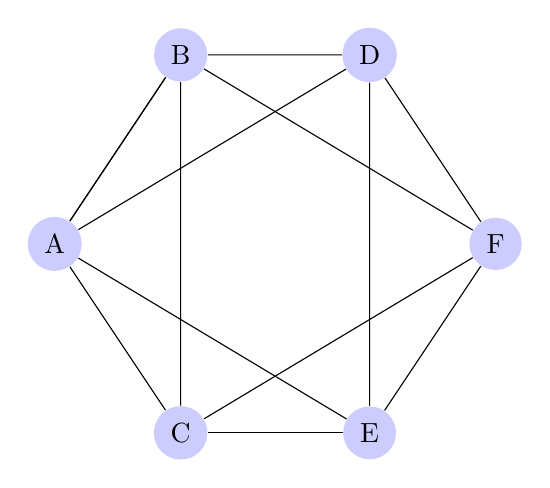
\begin{tikzpicture}
  [scale=.8,auto=left,every node/.style={circle,fill=blue!20}]
  \node (n1) at (2,4) {A};
  \node (n2) at (4,7) {B};
  \node (n3) at (4,1) {C};
  \node (n4) at (7,7) {D};
  \node (n5) at (7,1) {E};
  \node (n6) at (9,4) {F};

  \draw (n1) -- (n2);
  \draw (n1) -- (n2);
  \draw (n1) -- (n3);
  \draw (n1) -- (n4);
  \draw (n1) -- (n5);

  \draw (n2) -- (n3);
  \draw (n2) -- (n4);
  \draw (n2) -- (n6);

  \draw (n3) -- (n5);
  \draw (n3) -- (n6);

  \draw (n4) -- (n5);
  \draw (n4) -- (n6);

  \draw (n5) -- (n6);
\end{tikzpicture}
\caption{Grafo sin colorear}
\label{fig:graph}
\end{minipage}\hfill
\begin{minipage}{0.5\textwidth}
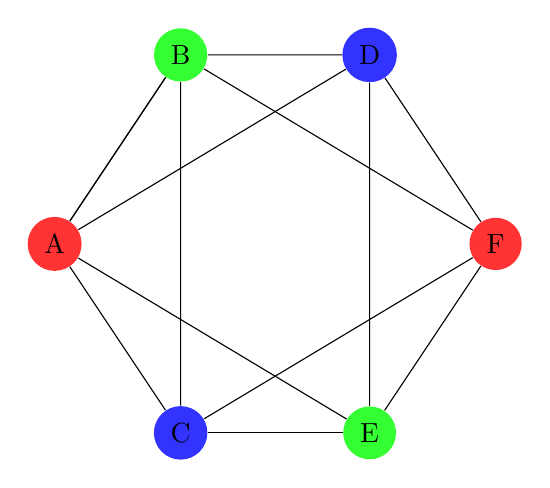
\begin{tikzpicture}
  [scale=.8,auto=left,every node/.style={circle}]
  \node[fill=red!80] (n1) at (2,4) {A};
  \node[fill=green!80] (n2) at (4,7) {B};
  \node[fill=blue!80] (n3) at (4,1) {C};
  \node[fill=blue!80] (n4) at (7,7) {D};
  \node[fill=green!80] (n5) at (7,1) {E};
  \node[fill=red!80] (n6) at (9,4) {F};

  \draw (n1) -- (n2);
  \draw (n1) -- (n2);
  \draw (n1) -- (n3);
  \draw (n1) -- (n4);
  \draw (n1) -- (n5);

  \draw (n2) -- (n3);
  \draw (n2) -- (n4);
  \draw (n2) -- (n6);

  \draw (n3) -- (n5);
  \draw (n3) -- (n6);

  \draw (n4) -- (n5);
  \draw (n4) -- (n6);

  \draw (n5) -- (n6);
\end{tikzpicture}
\caption{Grafo coloreado}
\label{fig:graph_color}
\end{minipage}
\end{figure}

\begin{figure}
\begin{align*}
    & A, B, C, D, E, F \in \{Red,\ Green,\ Blue\}\\
    \\
    & A \neq B \land A \neq C \land A \neq D \land A \neq E\\
    & B \neq C \land B \neq D \land B \neq E \land B \neq F\\
    & C \neq E \land C \neq F\\
    & D \neq E \land D \neq F\\
    & E \neq F
\end{align*}
\caption{Restricciones para la coloración del grafo}
\label{fig:g_col_csp}
\end{figure}

\begin{figure}
\begin{align*}
    (ar \lor ag \lor ab)\ \land\\
    \neg(ar \land ag)\ \land \neg(ar \land ab)\ \land \neg(ag \land ab)\ \land\\
    \neg(ar \land br)\ \land \neg(ar \land cr)\ \land \neg(ar \land dr)\ \land \neg(ar \land er)\ \land\\
    \neg(ag \land bg)\ \land \neg(ag \land cg)\ \land \neg(ag \land dg)\ \land \neg(ag \land eg)\ \land\\
    \neg(ab \land bb)\ \land \neg(ab \land cb)\ \land \neg(ab \land db)\ \land \neg(ab \land eb)\ \land\\
    \vdots
\end{align*}
\caption{Restricciones para la coloración del grafo en \sat}
\label{fig:g_col_sat}
\end{figure}

En la figura \ref{fig:g_col_sat} se construye una proposición lógica siguiendo una notación para el nombre de las variables donde la primera letra es el nodo en minúsculas y la segunda es el color, por ejemplo \textit{ar} es el nodo \textit{A} de color rojo. Solo se muestra el nodo \textit{A} pero sigue el mismo patrón para los otros nodos.

\subsection{Ocho reinas}

Otro ejemplo sería el problema de las ocho reinas, el cual resuleve el posicionamiento de ocho reinas en un tablero de ajedrez sin que ninguna de ellas este amenazando a otra. En la figura \ref{fig:queens} se puede ver una de las posibles soluciones a este problema.

\begin{figure}
\centering
\newgame
\fenboard{q7/6q1/4q3/7q/1q6/3q4/5q2/2q5 w - - 0 20}
\showboard
\caption{Solución al problema de las ocho reinas}
\label{fig:queens}
\end{figure}

Las restricciones que modelarían este problema como un \textit{CSP} serían las que se muestran en la figura \ref{fig:queens_csp}, se puede notar que las restricciones están definidas para el caso específico de las ocho reinas pero puede aplicar a $n$ dimesiones donde el tamaño del problema debe ser para $n > 3$.

\begin{figure}
\begin{align*}
    Q = \{1, 2, 3, \dots, 8\}\\
    \forall i \in Q \cdot x_i \in Q\\
    \forall i,j \in Q \cdot x_i \neq x_j\\
    \forall i,j \in Q \cdot x_i - x_j \neq i - j\\
    \forall i,j \in Q \cdot x_j - x_i \neq i - j
\end{align*}
\caption{Restricciones del problema de las ocho reinas como \textit{CSP}}
\label{fig:queens_csp}
\end{figure}

En el caso de \sat, la modelación se puede ver en la figura \ref{fig:queens_sat}. La notación que se usa para las variables nos indica la casilla del tablero en la posición $i,j$, donde $i$ es la fila y $j$ es la columna; o vice versa porque el problema es simétrico. Se pueden ver algunas condiciones para la fila y columna $1$ pero se deben especificar para todo el tablero, al final se definen las restricciones para la diagonal principal pero faltarían todas las diagonales posibles.

\begin{figure}
\begin{align*}
    (q_{11} \lor q_{12} \lor q_{13}\lor\dots\lor q_{18})\ \land\\
    \neg(q_{11} \land q_{12})\ \land\neg(q_{11} \land q_{13})\ \land\dots\land\neg(q_{11} \land q_{18})\ \land\\
    \neg(q_{12} \land q_{13})\ \land\dots\land\neg(q_{12} \land q_{18})\ \land\\
    \vdots\\
    \neg(q_{11} \land q_{21})\ \land\neg(q_{11} \land q_{31})\ \land\dots\land\neg(q_{11} \land q_{81})\ \land\\
    \neg(q_{21} \land q_{31})\ \land\dots\land\neg(q_{21} \land q_{81})\ \land\\
    \vdots\\
    \neg(q_{11} \land q_{22})\ \land\neg(q_{11} \land q_{33})\ \land\dots\land\neg(q_{11} \land q_{44})\ \land\\
    \neg(q_{22} \land q_{33})\ \land\dots\land\neg(q_{22} \land q_{44})\ \land\\
    \vdots
\end{align*}
\caption{Modelazión del problema de las ocho reinas para \sat}
\label{fig:queens_sat}
\end{figure}

\subsection{Sudoku}

Este problema establece una serie de restricciones sobre una matriz de $9\times9$, entre las cuales define que los posibles valores asignables a cada casilla son $1, 2, 3, \dots$ y $9$, además la matriz está separada en $9$ sub-matrices de $3\times 3$, dentro de ellas no pueden existir casillas con el mismo valor. Inicialmente se tiene la matriz parcialmente rellena con el objetivo de completarla, también se necesita que en cada fila y columna no exista un casilla con el mismo valor que otra. En la figura \ref{fig:sudoku} se puede ver un ejemplo de un sudoku.

\begin{figure}
  \centering
  \begin{tikzpicture}[scale=.5]
    \begin{scope}
      \draw (0, 0) grid (9, 9);
      \draw[very thick, scale=3] (0, 0) grid (3, 3);

      \setcounter{row}{1}
      \setrow { }{2}{ }  {5}{ }{1}  { }{9}{ }
      \setrow {8}{ }{ }  {2}{ }{3}  { }{ }{6}
      \setrow { }{3}{ }  { }{6}{ }  { }{7}{ }

      \setrow { }{ }{1}  { }{ }{ }  {6}{ }{ }
      \setrow {5}{4}{ }  { }{ }{ }  { }{1}{9}
      \setrow { }{ }{2}  { }{ }{ }  {7}{ }{ }

      \setrow { }{9}{ }  { }{3}{ }  { }{8}{ }
      \setrow {2}{ }{ }  {8}{ }{4}  { }{ }{7}
      \setrow { }{1}{ }  {9}{ }{7}  { }{6}{ }
    \end{scope}
  \end{tikzpicture}
  \caption{Ejemplo de un problema sudoku}
  \label{fig:sudoku}
\end{figure}

Se puede modelar como un \textit{CSP} estableciendo un dominio para los valores de las casillas, asignando un notación para las mismas, similar a un tablero de ajedrez y estableciendo las restricciones de las sub-matrices, filas, y columnas. Para traducirlo a \sat se deben establecer variables para cada casilla y los posibles valores que esta puede tomar, resultando en $729$ variables booleanas. Entonces, se podrían establecer las condiciones mediante fórmulas lógicas, separando las restricciones de forma similar a los ejemplos anteriores. Siendo un caso de prueba relativamente grande para atacar con \sat y en general para ser resuelto, siendo esta una motivación para implementar soluciones usando la \textit{GPU}, y poder abordar problemas de gran magnitud.

\section{Estructura del trabajo}

En los siguientes capítulos se describirá el proceso de implementación a una solución a \sat, comenzando por definir detalladamente esta representación junto a las implementaciones que se desarrollaron. Siguiendo con el diseño de una implementación que aproveche los recursos de la \textit{GPU}, a través de la plataforma OpenCL. Es importante resaltar, que para este trabajo trabajo se ha usado la versión \texttt{1.2}; en todo momento que se refiera a esta plataforma, la versión es tácita. También se describen otros soluciones que se implementaron, seguidas de los resultados experimentales obtenidos y un breve análisis de los mismos. Finalizando con las conclusiones y posibles trabajos futuros.
